% Options for packages loaded elsewhere
\PassOptionsToPackage{unicode}{hyperref}
\PassOptionsToPackage{hyphens}{url}
%
\documentclass[
  11pt,
]{article}
\usepackage{amsmath,amssymb}
\usepackage{iftex}
\ifPDFTeX
  \usepackage[T1]{fontenc}
  \usepackage[utf8]{inputenc}
  \usepackage{textcomp} % provide euro and other symbols
\else % if luatex or xetex
  \usepackage{unicode-math} % this also loads fontspec
  \defaultfontfeatures{Scale=MatchLowercase}
  \defaultfontfeatures[\rmfamily]{Ligatures=TeX,Scale=1}
\fi
\usepackage{lmodern}
\ifPDFTeX\else
  % xetex/luatex font selection
\fi
% Use upquote if available, for straight quotes in verbatim environments
\IfFileExists{upquote.sty}{\usepackage{upquote}}{}
\IfFileExists{microtype.sty}{% use microtype if available
  \usepackage[]{microtype}
  \UseMicrotypeSet[protrusion]{basicmath} % disable protrusion for tt fonts
}{}
\makeatletter
\@ifundefined{KOMAClassName}{% if non-KOMA class
  \IfFileExists{parskip.sty}{%
    \usepackage{parskip}
  }{% else
    \setlength{\parindent}{0pt}
    \setlength{\parskip}{6pt plus 2pt minus 1pt}}
}{% if KOMA class
  \KOMAoptions{parskip=half}}
\makeatother
\usepackage{xcolor}
\usepackage[left=1in,right=1in,top=1in,bottom=1in]{geometry}
\usepackage{color}
\usepackage{fancyvrb}
\newcommand{\VerbBar}{|}
\newcommand{\VERB}{\Verb[commandchars=\\\{\}]}
\DefineVerbatimEnvironment{Highlighting}{Verbatim}{commandchars=\\\{\}}
% Add ',fontsize=\small' for more characters per line
\usepackage{framed}
\definecolor{shadecolor}{RGB}{248,248,248}
\newenvironment{Shaded}{\begin{snugshade}}{\end{snugshade}}
\newcommand{\AlertTok}[1]{\textcolor[rgb]{0.94,0.16,0.16}{#1}}
\newcommand{\AnnotationTok}[1]{\textcolor[rgb]{0.56,0.35,0.01}{\textbf{\textit{#1}}}}
\newcommand{\AttributeTok}[1]{\textcolor[rgb]{0.13,0.29,0.53}{#1}}
\newcommand{\BaseNTok}[1]{\textcolor[rgb]{0.00,0.00,0.81}{#1}}
\newcommand{\BuiltInTok}[1]{#1}
\newcommand{\CharTok}[1]{\textcolor[rgb]{0.31,0.60,0.02}{#1}}
\newcommand{\CommentTok}[1]{\textcolor[rgb]{0.56,0.35,0.01}{\textit{#1}}}
\newcommand{\CommentVarTok}[1]{\textcolor[rgb]{0.56,0.35,0.01}{\textbf{\textit{#1}}}}
\newcommand{\ConstantTok}[1]{\textcolor[rgb]{0.56,0.35,0.01}{#1}}
\newcommand{\ControlFlowTok}[1]{\textcolor[rgb]{0.13,0.29,0.53}{\textbf{#1}}}
\newcommand{\DataTypeTok}[1]{\textcolor[rgb]{0.13,0.29,0.53}{#1}}
\newcommand{\DecValTok}[1]{\textcolor[rgb]{0.00,0.00,0.81}{#1}}
\newcommand{\DocumentationTok}[1]{\textcolor[rgb]{0.56,0.35,0.01}{\textbf{\textit{#1}}}}
\newcommand{\ErrorTok}[1]{\textcolor[rgb]{0.64,0.00,0.00}{\textbf{#1}}}
\newcommand{\ExtensionTok}[1]{#1}
\newcommand{\FloatTok}[1]{\textcolor[rgb]{0.00,0.00,0.81}{#1}}
\newcommand{\FunctionTok}[1]{\textcolor[rgb]{0.13,0.29,0.53}{\textbf{#1}}}
\newcommand{\ImportTok}[1]{#1}
\newcommand{\InformationTok}[1]{\textcolor[rgb]{0.56,0.35,0.01}{\textbf{\textit{#1}}}}
\newcommand{\KeywordTok}[1]{\textcolor[rgb]{0.13,0.29,0.53}{\textbf{#1}}}
\newcommand{\NormalTok}[1]{#1}
\newcommand{\OperatorTok}[1]{\textcolor[rgb]{0.81,0.36,0.00}{\textbf{#1}}}
\newcommand{\OtherTok}[1]{\textcolor[rgb]{0.56,0.35,0.01}{#1}}
\newcommand{\PreprocessorTok}[1]{\textcolor[rgb]{0.56,0.35,0.01}{\textit{#1}}}
\newcommand{\RegionMarkerTok}[1]{#1}
\newcommand{\SpecialCharTok}[1]{\textcolor[rgb]{0.81,0.36,0.00}{\textbf{#1}}}
\newcommand{\SpecialStringTok}[1]{\textcolor[rgb]{0.31,0.60,0.02}{#1}}
\newcommand{\StringTok}[1]{\textcolor[rgb]{0.31,0.60,0.02}{#1}}
\newcommand{\VariableTok}[1]{\textcolor[rgb]{0.00,0.00,0.00}{#1}}
\newcommand{\VerbatimStringTok}[1]{\textcolor[rgb]{0.31,0.60,0.02}{#1}}
\newcommand{\WarningTok}[1]{\textcolor[rgb]{0.56,0.35,0.01}{\textbf{\textit{#1}}}}
\usepackage{graphicx}
\makeatletter
\def\maxwidth{\ifdim\Gin@nat@width>\linewidth\linewidth\else\Gin@nat@width\fi}
\def\maxheight{\ifdim\Gin@nat@height>\textheight\textheight\else\Gin@nat@height\fi}
\makeatother
% Scale images if necessary, so that they will not overflow the page
% margins by default, and it is still possible to overwrite the defaults
% using explicit options in \includegraphics[width, height, ...]{}
\setkeys{Gin}{width=\maxwidth,height=\maxheight,keepaspectratio}
% Set default figure placement to htbp
\makeatletter
\def\fps@figure{htbp}
\makeatother
\setlength{\emergencystretch}{3em} % prevent overfull lines
\providecommand{\tightlist}{%
  \setlength{\itemsep}{0pt}\setlength{\parskip}{0pt}}
\setcounter{secnumdepth}{-\maxdimen} % remove section numbering
\usepackage{fvextra}
\DefineVerbatimEnvironment{Highlighting}{Verbatim}{breaklines, breakanywhere, commandchars=\\\{\}}
\usepackage{booktabs}
\usepackage{longtable}
\usepackage{array}
\usepackage{multirow}
\usepackage{wrapfig}
\usepackage{float}
\usepackage{colortbl}
\usepackage{pdflscape}
\usepackage{tabu}
\usepackage{threeparttable}
\usepackage{threeparttablex}
\usepackage[normalem]{ulem}
\usepackage{makecell}
\usepackage{xcolor}
\ifLuaTeX
  \usepackage{selnolig}  % disable illegal ligatures
\fi
\usepackage{bookmark}
\IfFileExists{xurl.sty}{\usepackage{xurl}}{} % add URL line breaks if available
\urlstyle{same}
\hypersetup{
  pdftitle={POL501 - Problem Set 3},
  pdfauthor={Solutions},
  hidelinks,
  pdfcreator={LaTeX via pandoc}}

\title{POL501 - Problem Set 3}
\author{Solutions}
\date{2024-12-04}

\begin{document}
\maketitle

{
\setcounter{tocdepth}{2}
\tableofcontents
}
\newpage

\section{Grading Criteria}\label{grading-criteria}

\begin{itemize}
\tightlist
\item
  There will be \textbf{four problem sets} throughout the semester,
  which together account for \textbf{25\% of the final course grade}.
\item
  The total possible score for these problem sets is \textbf{25 out of
  100 points} (with 100 points being the maximum course score).
\item
  This problem set has a maximum score of \textbf{6.5 points}.
\item
  \textbf{Scoring Breakdown}:

  \begin{itemize}
  \tightlist
  \item
    Each sub-letter in Question 1 is worth \textbf{0.5 point} (Total of
    2.5 points)
  \item
    Each sub-letter in Question 2 is worth \textbf{0.5 points} (Total of
    1.5 points)
  \item
    Each sub-letter in Question 3 is worth \textbf{0.5 points} (Total of
    2.5 points)
  \end{itemize}
\item
  \textbf{Grading Guidelines}:

  \begin{itemize}
  \tightlist
  \item
    Full credit will be awarded for fully correct answers that closely
    match the provided solutions included in this document.
  \item
    Partial credit will be given for incomplete or partially incorrect
    answers/justifications.
  \item
    \textbf{0 points} will be awarded for missing answers, answers with
    no justification, or entirely incorrect responses.
  \item
    Submissions without the RMD file will have point deductions.
  \end{itemize}
\end{itemize}

\newpage

\begin{center}\rule{0.5\linewidth}{0.5pt}\end{center}

\section{Question 1 - Solutions}\label{question-1---solutions}

\subsection{Preliminary Steps}\label{preliminary-steps}

\textbf{Important}:

\begin{itemize}
\tightlist
\item
  You must place this RMD file in the same folder in which you have the
  data.
\item
  Then, you will be able to load the dataset into memory. The name of
  the dataset as an R object is \texttt{df\_clean}.
\end{itemize}

As a preliminary recommended step, and to make sure we understand how
the variables are coded and their distribution, let's start by
describing the data using summary statistics.

\begin{Shaded}
\begin{Highlighting}[]
\NormalTok{sstats\_list }\OtherTok{\textless{}{-}} \FunctionTok{c}\NormalTok{(}\StringTok{\textquotesingle{}vars\textquotesingle{}}\NormalTok{, }\StringTok{\textquotesingle{}n\textquotesingle{}}\NormalTok{, }\StringTok{\textquotesingle{}mean\textquotesingle{}}\NormalTok{, }\StringTok{\textquotesingle{}sd\textquotesingle{}}\NormalTok{, }\StringTok{\textquotesingle{}median\textquotesingle{}}\NormalTok{, }\StringTok{\textquotesingle{}min\textquotesingle{}}\NormalTok{, }\StringTok{\textquotesingle{}max\textquotesingle{}}\NormalTok{)}
\FunctionTok{kable}\NormalTok{(}\FunctionTok{describe}\NormalTok{(df\_clean)[sstats\_list], }\AttributeTok{format=}\StringTok{\textquotesingle{}latex\textquotesingle{}}\NormalTok{)}
\end{Highlighting}
\end{Shaded}

\begin{tabular}{l|r|r|r|r|r|r|r}
\hline
  & vars & n & mean & sd & median & min & max\\
\hline
RESPID & 1 & 5199 & 9457.661281 & 5483.2245412 & 9464 & 2 & 18838\\
\hline
PARTY & 2 & 5199 & 2.177150 & 0.9685161 & 2 & 1 & 4\\
\hline
INTFREQ & 3 & 5199 & 1.810156 & 0.8919744 & 2 & 1 & 5\\
\hline
RADIO & 4 & 5199 & 1.219465 & 0.4139242 & 1 & 1 & 2\\
\hline
ECON1MOD & 5 & 5199 & 2.730140 & 0.8352547 & 3 & 1 & 4\\
\hline
INFRASPEND & 6 & 5199 & 2.151568 & 0.9420048 & 2 & 1 & 5\\
\hline
MOREGUNIMPACT & 7 & 5199 & 1.878631 & 0.8552866 & 2 & 1 & 3\\
\hline
CRIMESAFE & 8 & 5199 & 2.575303 & 0.8459974 & 3 & 1 & 5\\
\hline
\end{tabular}

Then, we define a user-defined function to compute confidence intervals.
The benefit of defining this function, is that we can then reuse it
multiple times just by providing new inputs.

\begin{Shaded}
\begin{Highlighting}[]
\CommentTok{\# Function to calculate confidence interval}
\NormalTok{confidence\_interval }\OtherTok{\textless{}{-}} \ControlFlowTok{function}\NormalTok{(data, var\_name, }\AttributeTok{confidence\_level =} \FloatTok{0.95}\NormalTok{, }\AttributeTok{method =} \StringTok{"t"}\NormalTok{) \{}

  \CommentTok{\# Extract the data column}
\NormalTok{  data\_column }\OtherTok{\textless{}{-}}\NormalTok{ data[[var\_name]]}
  
  \CommentTok{\# Validate inputs (method, var\_name)}
  \ControlFlowTok{if}\NormalTok{ (}\SpecialCharTok{!}\NormalTok{(method }\SpecialCharTok{\%in\%} \FunctionTok{c}\NormalTok{(}\StringTok{"t"}\NormalTok{, }\StringTok{"z"}\NormalTok{))) \{}
    \FunctionTok{stop}\NormalTok{(}\StringTok{"Method must be either \textquotesingle{}t\textquotesingle{} or \textquotesingle{}z\textquotesingle{}."}\NormalTok{)}
\NormalTok{  \}}
  \ControlFlowTok{if}\NormalTok{ (}\SpecialCharTok{!}\NormalTok{(var\_name }\SpecialCharTok{\%in\%} \FunctionTok{colnames}\NormalTok{(data))) \{}
    \FunctionTok{stop}\NormalTok{(}\StringTok{"var\_name must be the name of a column in the data frame."}\NormalTok{)}
\NormalTok{  \}}
  
  \CommentTok{\# Calculate sample statistics}
\NormalTok{  sample\_mean }\OtherTok{\textless{}{-}} \FunctionTok{mean}\NormalTok{(data\_column, }\AttributeTok{na.rm =} \ConstantTok{TRUE}\NormalTok{)}
\NormalTok{  sample\_sd }\OtherTok{\textless{}{-}} \FunctionTok{sd}\NormalTok{(data\_column, }\AttributeTok{na.rm =} \ConstantTok{TRUE}\NormalTok{)}
\NormalTok{  n }\OtherTok{\textless{}{-}} \FunctionTok{length}\NormalTok{(}\FunctionTok{na.omit}\NormalTok{(data\_column))}
\NormalTok{  standard\_error }\OtherTok{\textless{}{-}}\NormalTok{ sample\_sd }\SpecialCharTok{/} \FunctionTok{sqrt}\NormalTok{(n)}
  
  \CommentTok{\# Set alpha for confidence level}
\NormalTok{  alpha }\OtherTok{\textless{}{-}} \DecValTok{1} \SpecialCharTok{{-}}\NormalTok{ confidence\_level}
  
  \CommentTok{\# Calculate the critical value based on the selected method}
  \ControlFlowTok{if}\NormalTok{ (method }\SpecialCharTok{==} \StringTok{"t"}\NormalTok{) \{}
\NormalTok{    critical\_value }\OtherTok{\textless{}{-}} \FunctionTok{qt}\NormalTok{(}\DecValTok{1} \SpecialCharTok{{-}}\NormalTok{ alpha }\SpecialCharTok{/} \DecValTok{2}\NormalTok{, }\AttributeTok{df =}\NormalTok{ n }\SpecialCharTok{{-}} \DecValTok{1}\NormalTok{)  }\CommentTok{\# t{-}distribution critical value}
\NormalTok{  \} }\ControlFlowTok{else}\NormalTok{ \{}
\NormalTok{    critical\_value }\OtherTok{\textless{}{-}} \FunctionTok{qnorm}\NormalTok{(}\DecValTok{1} \SpecialCharTok{{-}}\NormalTok{ alpha }\SpecialCharTok{/} \DecValTok{2}\NormalTok{)  }\CommentTok{\# z{-}distribution critical value}
\NormalTok{  \}}
  
  \CommentTok{\# Calculate margin of error (MOE)}
\NormalTok{  margin\_of\_error }\OtherTok{\textless{}{-}}\NormalTok{ critical\_value }\SpecialCharTok{*}\NormalTok{ standard\_error}
  
  \CommentTok{\# Calculate confidence interval bounds}
\NormalTok{  lower\_bound }\OtherTok{\textless{}{-}}\NormalTok{ sample\_mean }\SpecialCharTok{{-}}\NormalTok{ margin\_of\_error}
\NormalTok{  upper\_bound }\OtherTok{\textless{}{-}}\NormalTok{ sample\_mean }\SpecialCharTok{+}\NormalTok{ margin\_of\_error}
  
  \CommentTok{\# Prepare output as a named vector}
\NormalTok{  output }\OtherTok{\textless{}{-}} \FunctionTok{c}\NormalTok{(}
    \StringTok{\textasciigrave{}}\AttributeTok{Sample Mean of}\StringTok{\textasciigrave{}} \OtherTok{=}\NormalTok{ var\_name,}
    \AttributeTok{Estimate =} \FunctionTok{round}\NormalTok{(sample\_mean, }\DecValTok{3}\NormalTok{),}
    \AttributeTok{MOE =} \FunctionTok{round}\NormalTok{(margin\_of\_error, }\DecValTok{3}\NormalTok{),}
    \StringTok{\textasciigrave{}}\AttributeTok{Lower CI Bound}\StringTok{\textasciigrave{}} \OtherTok{=} \FunctionTok{round}\NormalTok{(lower\_bound, }\DecValTok{3}\NormalTok{),}
    \StringTok{\textasciigrave{}}\AttributeTok{Upper CI Bound}\StringTok{\textasciigrave{}} \OtherTok{=} \FunctionTok{round}\NormalTok{(upper\_bound, }\DecValTok{3}\NormalTok{)}
\NormalTok{  )}

  \CommentTok{\# Return the result}
  \FunctionTok{return}\NormalTok{(output)}
\NormalTok{\}}
\end{Highlighting}
\end{Shaded}

\subsection{Answer to (1.a)}\label{answer-to-1.a}

First, recall the coding of \texttt{CRIMESAFE} responses. The question
asked: \textbf{\emph{How would you describe the area where you live, in
terms of crime?}}\$

\begin{itemize}
\tightlist
\item
  1 = Extremely safe;
\item
  2 = Very safe;
\item
  3 = Somewhat safe;
\item
  4 = Not too safe;
\item
  5 = Not at all safe
\end{itemize}

\begin{Shaded}
\begin{Highlighting}[]
\CommentTok{\# Question 1.a: Use the function \textasciigrave{}confidence\_interval\textasciigrave{} to compute the mean of \textasciigrave{}CRIMESAFE\textasciigrave{} with a 95\% confidence level. Interpret the confidence interval appropriately.}
\NormalTok{crimesafe\_CI\_z\_95 }\OtherTok{\textless{}{-}} \FunctionTok{confidence\_interval}\NormalTok{(}\AttributeTok{data=}\NormalTok{df\_clean, }
                                         \AttributeTok{var\_name=}\StringTok{\textquotesingle{}CRIMESAFE\textquotesingle{}}\NormalTok{, }
                                         \AttributeTok{confidence\_level =} \FloatTok{0.95}\NormalTok{, }\AttributeTok{method =} \StringTok{"t"}\NormalTok{)}
\FunctionTok{print}\NormalTok{(crimesafe\_CI\_z\_95)}
\end{Highlighting}
\end{Shaded}

\begin{verbatim}
## Sample Mean of       Estimate            MOE Lower CI Bound Upper CI Bound 
##    "CRIMESAFE"        "2.575"        "0.023"        "2.552"        "2.598"
\end{verbatim}

\begin{Shaded}
\begin{Highlighting}[]
\FunctionTok{kable}\NormalTok{(crimesafe\_CI\_z\_95, }\AttributeTok{format=}\StringTok{\textquotesingle{}latex\textquotesingle{}}\NormalTok{, }\AttributeTok{caption =} \StringTok{"95}\SpecialCharTok{\textbackslash{}\textbackslash{}}\StringTok{\% CI for the mean of \textasciigrave{}CRIMESAFE\textasciigrave{}"}\NormalTok{)}
\end{Highlighting}
\end{Shaded}

\begin{table}

\caption{\label{tab:q1-a}95\% CI for the mean of `CRIMESAFE`}
\centering
\begin{tabular}[t]{l|l}
\hline
  & x\\
\hline
Sample Mean of & CRIMESAFE\\
\hline
Estimate & 2.575\\
\hline
MOE & 0.023\\
\hline
Lower CI Bound & 2.552\\
\hline
Upper CI Bound & 2.598\\
\hline
\end{tabular}
\end{table}

\textbf{Explanation/Justification}: The average score for CRIMESAFE is
2.575, with a 95\% confidence interval ranging from 2.552 to 2.598. This
means we can be 95\% confident that the true average perception of
safety in the area falls within this range. Since the scale ranges from
1 (Extremely Safe) to 5 (Not at All Safe), a score of 2.575 indicates
that most people feel their area is somewhere between ``Very Safe'' and
``Somewhat Safe.'' The narrow margin of error (0.023) suggests the
estimate is precise, giving us strong confidence in this result.

\subsection{Answer to (1.b)}\label{answer-to-1.b}

\begin{Shaded}
\begin{Highlighting}[]
\CommentTok{\# Question 1.b: Use the function \textasciigrave{}confidence\_interval\textasciigrave{} to compute the mean of \textasciigrave{}CRIMESAFE\textasciigrave{} with a 99\% confidence level}
\NormalTok{crimesafe\_CI\_z\_99 }\OtherTok{\textless{}{-}} \FunctionTok{confidence\_interval}\NormalTok{(}\AttributeTok{data=}\NormalTok{df\_clean, }
                                         \AttributeTok{var\_name=}\StringTok{\textquotesingle{}CRIMESAFE\textquotesingle{}}\NormalTok{, }
                                         \AttributeTok{confidence\_level =} \FloatTok{0.99}\NormalTok{, }\AttributeTok{method =} \StringTok{"t"}\NormalTok{)}
\FunctionTok{print}\NormalTok{(crimesafe\_CI\_z\_99)}
\end{Highlighting}
\end{Shaded}

\begin{verbatim}
## Sample Mean of       Estimate            MOE Lower CI Bound Upper CI Bound 
##    "CRIMESAFE"        "2.575"         "0.03"        "2.545"        "2.606"
\end{verbatim}

\begin{Shaded}
\begin{Highlighting}[]
\FunctionTok{kable}\NormalTok{(crimesafe\_CI\_z\_99, }\AttributeTok{format=}\StringTok{\textquotesingle{}latex\textquotesingle{}}\NormalTok{,}\AttributeTok{caption =} \StringTok{"99}\SpecialCharTok{\textbackslash{}\textbackslash{}}\StringTok{\% CI for the mean of \textasciigrave{}CRIMESAFE\textasciigrave{}"}\NormalTok{)}
\end{Highlighting}
\end{Shaded}

\begin{table}

\caption{\label{tab:q1-b}99\% CI for the mean of `CRIMESAFE`}
\centering
\begin{tabular}[t]{l|l}
\hline
  & x\\
\hline
Sample Mean of & CRIMESAFE\\
\hline
Estimate & 2.575\\
\hline
MOE & 0.03\\
\hline
Lower CI Bound & 2.545\\
\hline
Upper CI Bound & 2.606\\
\hline
\end{tabular}
\end{table}

\textbf{Explanation/Justification}: The average score for CRIMESAFE is
2.575, with a 99\% confidence interval ranging from 2.545 to 2.606. This
means we can be 99\% confident that the true average perception of
safety in the area lies within this range. Similar to the 95\%
confidence interval, the score of 2.575 reflects that most people
perceive their neighborhood as between ``Very Safe'' and ``Somewhat
Safe.'' However, the wider margin of error (0.03) in the 99\% confidence
interval compared to the 95\% interval shows that increasing the
confidence level requires a broader range to ensure higher certainty.
This still indicates a generally positive perception of safety in the
community with a high degree of confidence.

\subsection{Answer to (1.c)}\label{answer-to-1.c}

\begin{Shaded}
\begin{Highlighting}[]
\CommentTok{\# Question 1.c: Use the \textasciigrave{}dplyr\textasciigrave{} command \textquotesingle{}filter\textquotesingle{} to create a data frame for the responses of Democrats and Republicans}
\CommentTok{\# Create one data frame for Democrats and another for Republicans}

\CommentTok{\# Let\textquotesingle{}s inspect the values of the variable \textasciigrave{}PARTY\textasciigrave{}}
\FunctionTok{table}\NormalTok{(df\_clean}\SpecialCharTok{$}\NormalTok{PARTY)}
\end{Highlighting}
\end{Shaded}

\begin{verbatim}
## 
##    1    2    3    4 
## 1514 1795 1345  545
\end{verbatim}

\begin{Shaded}
\begin{Highlighting}[]
\CommentTok{\# Filter rows and create subsamples}
\NormalTok{df\_dems }\OtherTok{\textless{}{-}}\NormalTok{ df\_clean }\SpecialCharTok{\%\textgreater{}\%}
  \FunctionTok{filter}\NormalTok{(PARTY}\SpecialCharTok{==}\DecValTok{2}\NormalTok{) }

\NormalTok{df\_rep }\OtherTok{\textless{}{-}}\NormalTok{ df\_clean }\SpecialCharTok{\%\textgreater{}\%}
  \FunctionTok{filter}\NormalTok{(PARTY}\SpecialCharTok{==}\DecValTok{1}\NormalTok{) }
\end{Highlighting}
\end{Shaded}

\textbf{Explanation/Justification}:

First, we recall that the coding for the responses for the
\texttt{PARTY} variable are:

\texttt{PARTY}. In politics today, do you consider yourself a\ldots{}

\begin{itemize}
\tightlist
\item
  1 = Republican;
\item
  2 = Democrat;
\item
  3 = Independent;
\item
  4 = Something else.
\end{itemize}

Thus, using \texttt{filter()} we select the rows matching Republicans
and Democrats. The data frame \texttt{df\_dems} includes rows where
\(PARTY=2\) which matches respondents who selected \(2 = Democrat\), and
the data frame \texttt{df\_reps} includes rows where \(PARTY=1\), which
corresponds to respondents who selected \(1 = Republican\).

\subsection{Answer to (1.d)}\label{answer-to-1.d}

\begin{Shaded}
\begin{Highlighting}[]
\CommentTok{\# Question 1.d: Compute the sample mean for \textasciigrave{}CRIMESAFE\textasciigrave{} and 95\% confidence intervals for Democrats and Republicans}
\NormalTok{crimesafe\_CI\_z\_95\_dems }\OtherTok{\textless{}{-}} \FunctionTok{confidence\_interval}\NormalTok{(}\AttributeTok{data=}\NormalTok{df\_dems, }
                                         \AttributeTok{var\_name=}\StringTok{\textquotesingle{}CRIMESAFE\textquotesingle{}}\NormalTok{, }
                                         \AttributeTok{confidence\_level =} \FloatTok{0.95}\NormalTok{, }\AttributeTok{method =} \StringTok{"t"}\NormalTok{)}
\FunctionTok{cat}\NormalTok{(}\StringTok{\textquotesingle{}}\SpecialCharTok{\textbackslash{}n}\StringTok{Results for Democrats:}\SpecialCharTok{\textbackslash{}n}\StringTok{\textquotesingle{}}\NormalTok{)}
\end{Highlighting}
\end{Shaded}

\begin{verbatim}
## 
## Results for Democrats:
\end{verbatim}

\begin{Shaded}
\begin{Highlighting}[]
\FunctionTok{print}\NormalTok{(crimesafe\_CI\_z\_95\_dems)}
\end{Highlighting}
\end{Shaded}

\begin{verbatim}
## Sample Mean of       Estimate            MOE Lower CI Bound Upper CI Bound 
##    "CRIMESAFE"        "2.526"         "0.04"        "2.486"        "2.566"
\end{verbatim}

\begin{Shaded}
\begin{Highlighting}[]
\FunctionTok{kable}\NormalTok{(crimesafe\_CI\_z\_95\_dems, }\AttributeTok{format=}\StringTok{\textquotesingle{}latex\textquotesingle{}}\NormalTok{, }\AttributeTok{caption =} \StringTok{"95}\SpecialCharTok{\textbackslash{}\textbackslash{}}\StringTok{\% CI for the mean of \textasciigrave{}CRIMESAFE\textasciigrave{} among Democrats"}\NormalTok{)}
\end{Highlighting}
\end{Shaded}

\begin{table}

\caption{\label{tab:q1-d-part1}95\% CI for the mean of `CRIMESAFE` among Democrats}
\centering
\begin{tabular}[t]{l|l}
\hline
  & x\\
\hline
Sample Mean of & CRIMESAFE\\
\hline
Estimate & 2.526\\
\hline
MOE & 0.04\\
\hline
Lower CI Bound & 2.486\\
\hline
Upper CI Bound & 2.566\\
\hline
\end{tabular}
\end{table}

\begin{Shaded}
\begin{Highlighting}[]
\NormalTok{crimesafe\_CI\_z\_95\_reps }\OtherTok{\textless{}{-}} \FunctionTok{confidence\_interval}\NormalTok{(}\AttributeTok{data=}\NormalTok{df\_rep, }
                                         \AttributeTok{var\_name=}\StringTok{\textquotesingle{}CRIMESAFE\textquotesingle{}}\NormalTok{, }
                                         \AttributeTok{confidence\_level =} \FloatTok{0.95}\NormalTok{, }\AttributeTok{method =} \StringTok{"t"}\NormalTok{)}
\FunctionTok{cat}\NormalTok{(}\StringTok{\textquotesingle{}}\SpecialCharTok{\textbackslash{}n}\StringTok{Results for Republicans:}\SpecialCharTok{\textbackslash{}n}\StringTok{\textquotesingle{}}\NormalTok{)}
\end{Highlighting}
\end{Shaded}

\begin{verbatim}
## 
## Results for Republicans:
\end{verbatim}

\begin{Shaded}
\begin{Highlighting}[]
\FunctionTok{print}\NormalTok{(crimesafe\_CI\_z\_95\_reps)}
\end{Highlighting}
\end{Shaded}

\begin{verbatim}
## Sample Mean of       Estimate            MOE Lower CI Bound Upper CI Bound 
##    "CRIMESAFE"        "2.596"        "0.041"        "2.556"        "2.637"
\end{verbatim}

\begin{Shaded}
\begin{Highlighting}[]
\FunctionTok{kable}\NormalTok{(crimesafe\_CI\_z\_95\_reps, }\AttributeTok{format=}\StringTok{\textquotesingle{}latex\textquotesingle{}}\NormalTok{, }\AttributeTok{caption =} \StringTok{"95}\SpecialCharTok{\textbackslash{}\textbackslash{}}\StringTok{\% CI for the mean of \textasciigrave{}CRIMESAFE\textasciigrave{} among Republicans"}\NormalTok{)}
\end{Highlighting}
\end{Shaded}

\begin{table}

\caption{\label{tab:q1-d-part2}95\% CI for the mean of `CRIMESAFE` among Republicans}
\centering
\begin{tabular}[t]{l|l}
\hline
  & x\\
\hline
Sample Mean of & CRIMESAFE\\
\hline
Estimate & 2.596\\
\hline
MOE & 0.041\\
\hline
Lower CI Bound & 2.556\\
\hline
Upper CI Bound & 2.637\\
\hline
\end{tabular}
\end{table}

\textbf{Explanation/Justification}: The results show that Democrats have
an average CRIMESAFE score of 2.526, with a 95\% confidence interval of
{[}2.486, 2.566{]}, indicating they perceive their neighborhoods as
leaning towards ``Very Safe'' to ``Somewhat Safe.'' Republicans, on the
other hand, have a slightly higher average score of 2.596, with a 95\%
confidence interval of {[}2.556, 2.637{]}, suggesting they also perceive
their neighborhoods as ``Very Safe'' to ``Somewhat Safe,'' but slightly
less safe compared to Democrats.

\subsection{Answer to (1.e)}\label{answer-to-1.e}

\begin{Shaded}
\begin{Highlighting}[]
\CommentTok{\# Question 1.e: Create a data frame with the results of (1.d) and plot the results}
\CommentTok{\# Extract the values and combine them into a data frame for plotting}
\NormalTok{combined\_crimesafe\_CI\_95 }\OtherTok{\textless{}{-}} \FunctionTok{cbind}\NormalTok{(}\FunctionTok{c}\NormalTok{(}\AttributeTok{Group =} \StringTok{\textquotesingle{}Democrats\textquotesingle{}}\NormalTok{, crimesafe\_CI\_z\_95\_dems),}
                                  \FunctionTok{c}\NormalTok{(}\AttributeTok{Group =} \StringTok{\textquotesingle{}Republicans\textquotesingle{}}\NormalTok{, crimesafe\_CI\_z\_95\_reps))}

\CommentTok{\# Convert the combined matrix into a data frame with proper column names}
\NormalTok{df\_combined\_CI }\OtherTok{\textless{}{-}} \FunctionTok{as.data.frame}\NormalTok{(}\FunctionTok{t}\NormalTok{(combined\_crimesafe\_CI\_95), }\AttributeTok{stringsAsFactors =} \ConstantTok{FALSE}\NormalTok{)}

\CommentTok{\# Rename columns for clarity}
\FunctionTok{colnames}\NormalTok{(df\_combined\_CI) }\OtherTok{\textless{}{-}} \FunctionTok{c}\NormalTok{(}\StringTok{"Group"}\NormalTok{, }\StringTok{"Sample\_Mean"}\NormalTok{, }\StringTok{"Estimate"}\NormalTok{, }\StringTok{"MOE"}\NormalTok{, }\StringTok{"Lower"}\NormalTok{, }\StringTok{"Upper"}\NormalTok{)}

\CommentTok{\# Convert relevant columns to numeric}
\NormalTok{df\_combined\_CI }\OtherTok{\textless{}{-}}\NormalTok{ df\_combined\_CI }\SpecialCharTok{\%\textgreater{}\%}
  \FunctionTok{mutate}\NormalTok{(}\AttributeTok{Estimate =} \FunctionTok{as.numeric}\NormalTok{(Estimate),}
         \AttributeTok{Lower =} \FunctionTok{as.numeric}\NormalTok{(Lower),}
         \AttributeTok{Upper =} \FunctionTok{as.numeric}\NormalTok{(Upper))}

\CommentTok{\# Plot using ggplot2 with a dot and whiskers for confidence interval}
\FunctionTok{ggplot}\NormalTok{(df\_combined\_CI, }\FunctionTok{aes}\NormalTok{(}\AttributeTok{x =}\NormalTok{ Group, }\AttributeTok{y =}\NormalTok{ Estimate)) }\SpecialCharTok{+}
  \FunctionTok{geom\_errorbar}\NormalTok{(}\FunctionTok{aes}\NormalTok{(}\AttributeTok{ymin =}\NormalTok{ Lower, }\AttributeTok{ymax =}\NormalTok{ Upper), }\AttributeTok{width =} \FloatTok{0.1}\NormalTok{, }\AttributeTok{color =} \StringTok{"steelblue"}\NormalTok{) }\SpecialCharTok{+}  \CommentTok{\# Whiskers for CI}
  \FunctionTok{geom\_point}\NormalTok{(}\AttributeTok{size =} \DecValTok{3}\NormalTok{, }\AttributeTok{color =} \StringTok{"navyblue"}\NormalTok{) }\SpecialCharTok{+}  \CommentTok{\# Dot for the sample mean}
  \FunctionTok{labs}\NormalTok{(}
    \AttributeTok{title =} \StringTok{"Mean Perception of Community Safety with 95\% Confidence Interval"}\NormalTok{,}
    \AttributeTok{x =} \StringTok{"Political Affiliation"}\NormalTok{,}
    \AttributeTok{y =} \StringTok{"Perception of Community Safety (CRIMESAFE)"}
\NormalTok{  ) }\SpecialCharTok{+}
  \FunctionTok{theme\_minimal}\NormalTok{() }\SpecialCharTok{+} 
  \FunctionTok{ylim}\NormalTok{(}\FloatTok{2.4}\NormalTok{, }\FloatTok{2.7}\NormalTok{)  }\CommentTok{\# Set the y{-}axis limits here}
\end{Highlighting}
\end{Shaded}

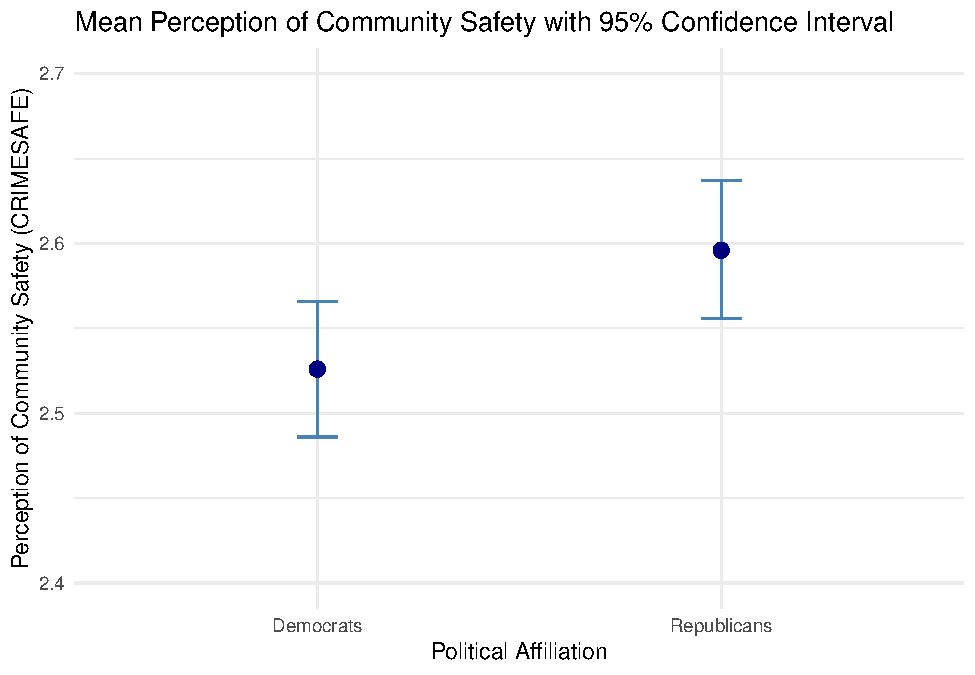
\includegraphics{Answers-PS3_files/figure-latex/q1-e-1.pdf}

\textbf{Explanation/Justification}: The plot shows that the 95\%
confidence intervals for Democrats ({[}2.486, 2.566{]}) and Republicans
({[}2.556, 2.637{]}) represent the range within which their true mean
perceptions of neighborhood safety likely fall. While these intervals
overlap slightly, this does not automatically imply that the difference
in their true means is not statistically significant. Intuitively, a
smaller overlap does indicate a lower likelihood that the true means of
the two groups are the same. Yet, overlap of confidence intervals is not
a definitive test of significance and can lead to misinterpretation. To
properly assess whether the difference in perceptions is statistically
meaningful, a confidence interval for the difference in means between
the two groups should be calculated.

\begin{center}\rule{0.5\linewidth}{0.5pt}\end{center}

\section{Question 2 - Solutions}\label{question-2---solutions}

This question follows the previous one and now focuses on inference for
proportions.

Recall the coding of \texttt{CRIMESAFE} responses. The question asked:
\textbf{\emph{How would you describe the area where you live, in terms
of crime?}}\$

\begin{itemize}
\tightlist
\item
  1 = Extremely safe;
\item
  2 = Very safe;
\item
  3 = Somewhat safe;
\item
  4 = Not too safe;
\item
  5 = Not at all safe
\end{itemize}

\subsection{Answer to (2.a)}\label{answer-to-2.a}

\begin{Shaded}
\begin{Highlighting}[]
\CommentTok{\# Question 2.a: Create a new variable in the dataframe \textasciigrave{}df\_clean\textasciigrave{} that equals 1 if the respondent selected}
\CommentTok{\# "Not too safe" (=4) or "Not at all safe" (=5), and zero otherwise. Then, recreate the subsample data frames for Democrats and Republicans.}
\CommentTok{\# Finally, interpret the mean of this variable.}

\NormalTok{df\_clean }\OtherTok{\textless{}{-}}\NormalTok{ df\_clean }\SpecialCharTok{\%\textgreater{}\%}
  \FunctionTok{mutate}\NormalTok{(}
    \AttributeTok{notsafe\_binary =} \FunctionTok{if\_else}\NormalTok{(CRIMESAFE }\SpecialCharTok{\%in\%} \FunctionTok{c}\NormalTok{(}\DecValTok{4}\NormalTok{, }\DecValTok{5}\NormalTok{), }\DecValTok{1}\NormalTok{, }\DecValTok{0}\NormalTok{)}
\NormalTok{  )}

\CommentTok{\# Re{-}Create subsamples for Democrats and Republicans (Now the subsamples include the new variable)}
\NormalTok{df\_dems }\OtherTok{\textless{}{-}}\NormalTok{ df\_clean }\SpecialCharTok{\%\textgreater{}\%}
  \FunctionTok{filter}\NormalTok{(PARTY}\SpecialCharTok{==}\DecValTok{2}\NormalTok{) }

\NormalTok{df\_rep }\OtherTok{\textless{}{-}}\NormalTok{ df\_clean }\SpecialCharTok{\%\textgreater{}\%}
  \FunctionTok{filter}\NormalTok{(PARTY}\SpecialCharTok{==}\DecValTok{1}\NormalTok{) }

\CommentTok{\# Describe the mean of the new variable {-} entire sample}
\FunctionTok{print}\NormalTok{(}\StringTok{"Proportion of Respondents Who Selected \textasciigrave{}Not too safe\textasciigrave{} OR \textasciigrave{}Not at all safe\textasciigrave{} (entire sample):"}\NormalTok{)}
\end{Highlighting}
\end{Shaded}

\begin{verbatim}
## [1] "Proportion of Respondents Who Selected `Not too safe` OR `Not at all safe` (entire sample):"
\end{verbatim}

\begin{Shaded}
\begin{Highlighting}[]
\FunctionTok{mean}\NormalTok{(df\_clean}\SpecialCharTok{$}\NormalTok{notsafe\_binary)}
\end{Highlighting}
\end{Shaded}

\begin{verbatim}
## [1] 0.107136
\end{verbatim}

\begin{Shaded}
\begin{Highlighting}[]
\CommentTok{\# Describe the mean of the new variable for Democrats}
\FunctionTok{print}\NormalTok{(}\StringTok{"Proportion of Democrats Who Selected \textasciigrave{}Not too safe\textasciigrave{} OR \textasciigrave{}Not at all safe\textasciigrave{}:"}\NormalTok{)}
\end{Highlighting}
\end{Shaded}

\begin{verbatim}
## [1] "Proportion of Democrats Who Selected `Not too safe` OR `Not at all safe`:"
\end{verbatim}

\begin{Shaded}
\begin{Highlighting}[]
\FunctionTok{mean}\NormalTok{(df\_dems}\SpecialCharTok{$}\NormalTok{notsafe\_binary)}
\end{Highlighting}
\end{Shaded}

\begin{verbatim}
## [1] 0.1097493
\end{verbatim}

\begin{Shaded}
\begin{Highlighting}[]
\CommentTok{\# Describe the mean of the new variable for Republicans}
\FunctionTok{print}\NormalTok{(}\StringTok{"Proportion of Republicans Who Selected \textasciigrave{}Not too safe\textasciigrave{} OR \textasciigrave{}Not at all safe\textasciigrave{}:"}\NormalTok{)}
\end{Highlighting}
\end{Shaded}

\begin{verbatim}
## [1] "Proportion of Republicans Who Selected `Not too safe` OR `Not at all safe`:"
\end{verbatim}

\begin{Shaded}
\begin{Highlighting}[]
\FunctionTok{mean}\NormalTok{(df\_rep}\SpecialCharTok{$}\NormalTok{notsafe\_binary)}
\end{Highlighting}
\end{Shaded}

\begin{verbatim}
## [1] 0.0984148
\end{verbatim}

\begin{Shaded}
\begin{Highlighting}[]
\CommentTok{\# Create a summary dataframe}
\NormalTok{summary\_df }\OtherTok{\textless{}{-}} \FunctionTok{data.frame}\NormalTok{(}
  \AttributeTok{Group =} \FunctionTok{c}\NormalTok{(}\StringTok{"Entire Sample"}\NormalTok{, }\StringTok{"Democrats"}\NormalTok{, }\StringTok{"Republicans"}\NormalTok{),}
  \AttributeTok{Proportion =} \FunctionTok{c}\NormalTok{(}\StringTok{\textquotesingle{}mean\_fullsample\textquotesingle{}}\OtherTok{=}\FunctionTok{mean}\NormalTok{(df\_clean}\SpecialCharTok{$}\NormalTok{notsafe\_binary), }
                 \StringTok{\textquotesingle{}mean\_dems\textquotesingle{}}\OtherTok{=}\FunctionTok{mean}\NormalTok{(df\_dems}\SpecialCharTok{$}\NormalTok{notsafe\_binary), }
                 \StringTok{\textquotesingle{}mean\_reps\textquotesingle{}}\OtherTok{=}\FunctionTok{mean}\NormalTok{(df\_rep}\SpecialCharTok{$}\NormalTok{notsafe\_binary))}
\NormalTok{)}
\FunctionTok{rownames}\NormalTok{(summary\_df) }\OtherTok{\textless{}{-}} \ConstantTok{NULL} \CommentTok{\# Remove row "ID names"}
\NormalTok{summary\_df}\SpecialCharTok{$}\NormalTok{Proportion }\OtherTok{\textless{}{-}} \FunctionTok{round}\NormalTok{(summary\_df}\SpecialCharTok{$}\NormalTok{Proportion,}\DecValTok{3}\NormalTok{) }\CommentTok{\# round values}

\CommentTok{\# Use kable to display the dataframe}
\FunctionTok{print}\NormalTok{(summary\_df)}
\end{Highlighting}
\end{Shaded}

\begin{verbatim}
##           Group Proportion
## 1 Entire Sample      0.107
## 2     Democrats      0.110
## 3   Republicans      0.098
\end{verbatim}

\begin{Shaded}
\begin{Highlighting}[]
\FunctionTok{kable}\NormalTok{(summary\_df, }\AttributeTok{caption =} \StringTok{"Proportion of Respondents Who Selected \textasciigrave{}Not too safe\textasciigrave{} OR \textasciigrave{}Not at all safe\textasciigrave{}"}\NormalTok{, }\AttributeTok{format=}\StringTok{\textquotesingle{}latex\textquotesingle{}}\NormalTok{)}
\end{Highlighting}
\end{Shaded}

\begin{table}

\caption{\label{tab:q2-a}Proportion of Respondents Who Selected `Not too safe` OR `Not at all safe`}
\centering
\begin{tabular}[t]{l|r}
\hline
Group & Proportion\\
\hline
Entire Sample & 0.107\\
\hline
Democrats & 0.110\\
\hline
Republicans & 0.098\\
\hline
\end{tabular}
\end{table}

\textbf{Explanation/Justification}: The sample mean of the
\texttt{notsafe\_binary} variable represents the proportion of
respondents who perceive their neighborhoods as ``Not too safe'' or
``Not at all safe.'' For the entire sample, the proportion is
\textbf{0.107}, indicating that approximately 10.7\% of all respondents
feel their neighborhoods are unsafe. Among Democrats, the proportion is
slightly higher at \textbf{0.110}, meaning about 11.0\% of Democrats
perceive their neighborhoods as unsafe. For Republicans, the proportion
is slightly lower at \textbf{0.098}, with only 9.8\% expressing similar
concerns. These results suggest that Democrats are slightly more likely
than Republicans to feel unsafe in their neighborhoods, but overall, the
proportions are relatively small in both groups, indicating that the
majority of respondents from both political affiliations perceive their
neighborhoods as relatively safe.

\subsection{Answer to (2.b)}\label{answer-to-2.b}

\begin{Shaded}
\begin{Highlighting}[]
\CommentTok{\# Question 2.b: Using the subsample for Democrats, compute the p{-}value with the null hypothesis}
\CommentTok{\# that the true proportion for Democrats differs from the sample proportion for Republicans.}
\CommentTok{\# EXPLAIN AND INTERPRET THE RESULTS}

\NormalTok{prop\_null\_hypothesis }\OtherTok{\textless{}{-}} \FunctionTok{mean}\NormalTok{(df\_rep}\SpecialCharTok{$}\NormalTok{notsafe\_binary) }\CommentTok{\# hypothesis = the sample prop for reps}
\NormalTok{n\_sample\_size }\OtherTok{\textless{}{-}} \FunctionTok{nrow}\NormalTok{(df\_dems)}

\CommentTok{\# Calculate the standard DEVIATION for the null hypothesis (replace with the correct formula)}
\NormalTok{SD\_null\_hypot }\OtherTok{\textless{}{-}} \FunctionTok{sqrt}\NormalTok{(prop\_null\_hypothesis}\SpecialCharTok{*}\NormalTok{(}\DecValTok{1}\SpecialCharTok{{-}}\NormalTok{prop\_null\_hypothesis))}
  
\CommentTok{\# Run the z{-}test to test if the mean is significantly different from the sample proportion for Republicans}
\CommentTok{\#   The function will compute in the background the correct Standard Error.}
\NormalTok{z\_test\_result }\OtherTok{\textless{}{-}} \FunctionTok{z.test}\NormalTok{(}
  \AttributeTok{x =}\NormalTok{ df\_dems}\SpecialCharTok{$}\NormalTok{notsafe\_binary, }\CommentTok{\# Here we declare the variable for our sample, i.e., democrats}
  \AttributeTok{mu =}\NormalTok{ prop\_null\_hypothesis,  }\CommentTok{\# Hypothesized population mean}
  \AttributeTok{sigma.x =}\NormalTok{ SD\_null\_hypot  }\CommentTok{\# Population standard DEVIATION (given H0)}
\NormalTok{)}

\CommentTok{\# Print the z{-}test result}
\FunctionTok{print}\NormalTok{(z\_test\_result)}
\end{Highlighting}
\end{Shaded}

\begin{verbatim}
## 
##  One-sample z-Test
## 
## data:  df_dems$notsafe_binary
## z = 1.6121, p-value = 0.1069
## alternative hypothesis: true mean is not equal to 0.0984148
## 95 percent confidence interval:
##  0.0959693 0.1235293
## sample estimates:
## mean of x 
## 0.1097493
\end{verbatim}

\textbf{Explanation/Justification}: For the Democratic subsample, the
z-test results in a z-value of \textbf{1.6121} and a p-value of
\textbf{0.1069}. Since the p-value is greater than both the 5\%
(\(0.05\)) and 1\% (\(0.01\)) significance levels, we fail to reject the
null hypothesis. This means there is insufficient evidence to conclude
that the true proportion of Democrats who feel unsafe is significantly
different from the sample proportion observed for Republicans.

\subsection{Answer to (2.c)}\label{answer-to-2.c}

\begin{Shaded}
\begin{Highlighting}[]
\CommentTok{\# Question 2.c: Using the REPUBLICANS subsample, compute the p{-}value with the null hypothesis}
\CommentTok{\# that the true proportion differs from the estimated sample proportion for Democrats.}
\CommentTok{\# EXPLAIN AND INTERPRET THE RESULTS}

\NormalTok{prop\_null\_hypothesis }\OtherTok{\textless{}{-}} \FunctionTok{mean}\NormalTok{(df\_dems}\SpecialCharTok{$}\NormalTok{notsafe\_binary)}
\NormalTok{n\_sample\_size }\OtherTok{\textless{}{-}} \FunctionTok{nrow}\NormalTok{(df\_rep) }\CommentTok{\# UPDATED CODE LINE}

\CommentTok{\# Calculate the standard DEVIATION for the null hypothesis (replace with the correct formula)}
\NormalTok{SD\_null\_hypot }\OtherTok{\textless{}{-}} \FunctionTok{sqrt}\NormalTok{(prop\_null\_hypothesis}\SpecialCharTok{*}\NormalTok{(}\DecValTok{1}\SpecialCharTok{{-}}\NormalTok{prop\_null\_hypothesis))}
  
\CommentTok{\# Run the z{-}test to test if the mean is significantly different from the sample proportion for Democrats}
\NormalTok{z\_test\_result }\OtherTok{\textless{}{-}} \FunctionTok{z.test}\NormalTok{(}
  \AttributeTok{x =}\NormalTok{ df\_rep}\SpecialCharTok{$}\NormalTok{notsafe\_binary, }\CommentTok{\# Here we declare the variable for our sample}
  \AttributeTok{mu =}\NormalTok{ prop\_null\_hypothesis,  }\CommentTok{\# Hypothesized population mean}
  \AttributeTok{sigma.x =}\NormalTok{ SD\_null\_hypot  }\CommentTok{\# Population standard DEVIATION (assuming known)}
\NormalTok{)}

\CommentTok{\# Print the z{-}test result}
\FunctionTok{print}\NormalTok{(z\_test\_result)}
\end{Highlighting}
\end{Shaded}

\begin{verbatim}
## 
##  One-sample z-Test
## 
## data:  df_rep$notsafe_binary
## z = -1.4109, p-value = 0.1583
## alternative hypothesis: true mean is not equal to 0.1097493
## 95 percent confidence interval:
##  0.08266981 0.11415978
## sample estimates:
## mean of x 
## 0.0984148
\end{verbatim}

\textbf{Explanation/Justification}: For the Republican subsample, the
z-test yields a z-value of \textbf{-1.4109} and a p-value of
\textbf{0.1583}. Since the p-value is greater than both the 5\%
(\(0.05\)) and 1\% (\(0.01\)) significance levels, we fail to reject the
null hypothesis. This indicates there is insufficient evidence to
conclude that the true proportion of Republicans who feel unsafe is
significantly different from the sample proportion observed for
Democrats.

\begin{center}\rule{0.5\linewidth}{0.5pt}\end{center}

\section{Question 3 - Solutions}\label{question-3---solutions}

This question introduces hypothesis testing using a mock dataset for
proportions without relying on any specialized packages. In this
question you will test the null hypothesis that the true population
proportion is 0.43 against the alternative that it is different, using a
1\% significance level.

\subsection{Preliminary Steps}\label{preliminary-steps-1}

We will generate a new mock dataset for this question. We set a seed
equal to 12345 to ensure reproducibility and create the mock dataset.
Also, we will set up the simulated data using a bernoulli random
variable generator with a true proportion of success equal to 0.44. We
will use a sample size of 35 observations.

\textbf{Don't modify this chunk:}

\begin{Shaded}
\begin{Highlighting}[]
\CommentTok{\# Set seed for reproducibility}
\FunctionTok{set.seed}\NormalTok{(}\DecValTok{12345}\NormalTok{)}

\CommentTok{\# Create a mock dataset with 35 respondents where each respondent either supports (1) or does not support (0) a specific policy}
\NormalTok{respondents }\OtherTok{\textless{}{-}} \DecValTok{35}
\NormalTok{true\_prop }\OtherTok{\textless{}{-}} \FloatTok{0.44}
\NormalTok{mock\_data\_q3 }\OtherTok{\textless{}{-}} \FunctionTok{data.frame}\NormalTok{(}\AttributeTok{support\_policy =} \FunctionTok{rbinom}\NormalTok{(}\AttributeTok{n=}\NormalTok{respondents, }\AttributeTok{size=}\DecValTok{1}\NormalTok{, true\_prop))  }\CommentTok{\# size=1 means one trial, hence we are drawing \textquotesingle{}n\textquotesingle{} bernoulli random variables.}

\CommentTok{\# Visualize the first few rows of the dataset}
\FunctionTok{head}\NormalTok{(mock\_data\_q3)}
\end{Highlighting}
\end{Shaded}

\begin{verbatim}
##   support_policy
## 1              1
## 2              1
## 3              1
## 4              1
## 5              0
## 6              0
\end{verbatim}

\subsection{Answer to (3.a)}\label{answer-to-3.a}

First, calculate the sample proportion and the standard error.

\begin{Shaded}
\begin{Highlighting}[]
\CommentTok{\# Calculate the sample proportion}
\NormalTok{p\_hat }\OtherTok{\textless{}{-}} \FunctionTok{mean}\NormalTok{(mock\_data\_q3}\SpecialCharTok{$}\NormalTok{support\_policy) }\CommentTok{\# Observed Sample Proportion}

\CommentTok{\# Define the null hypothesis proportion}
\NormalTok{p\_0 }\OtherTok{\textless{}{-}} \FloatTok{0.43}

\CommentTok{\# Compute the sample size }
\NormalTok{n }\OtherTok{\textless{}{-}} \FunctionTok{nrow}\NormalTok{(mock\_data\_q3)}

\CommentTok{\# Calculate the standard ERROR under the null (Appropiate SE assuming H0 is true)}
\NormalTok{standard\_error\_null\_hypothesis }\OtherTok{\textless{}{-}} \FunctionTok{sqrt}\NormalTok{( ( p\_0}\SpecialCharTok{*}\NormalTok{(}\DecValTok{1} \SpecialCharTok{{-}}\NormalTok{ p\_0) )}\SpecialCharTok{/}\NormalTok{n )  }\CommentTok{\# SE assuming the null hypothesis}

\CommentTok{\# Print the results}
\FunctionTok{cat}\NormalTok{(}\StringTok{"Sample Proportion: "}\NormalTok{, }\FunctionTok{round}\NormalTok{(p\_hat, }\DecValTok{3}\NormalTok{), }\StringTok{"}\SpecialCharTok{\textbackslash{}n}\StringTok{"}\NormalTok{)}
\end{Highlighting}
\end{Shaded}

\begin{verbatim}
## Sample Proportion:  0.4
\end{verbatim}

\begin{Shaded}
\begin{Highlighting}[]
\FunctionTok{cat}\NormalTok{(}\StringTok{"Standard Error: "}\NormalTok{, }\FunctionTok{round}\NormalTok{(standard\_error\_null\_hypothesis, }\DecValTok{3}\NormalTok{), }\StringTok{"}\SpecialCharTok{\textbackslash{}n}\StringTok{"}\NormalTok{)}
\end{Highlighting}
\end{Shaded}

\begin{verbatim}
## Standard Error:  0.084
\end{verbatim}

\textbf{Explanation/Justification}: The sample proportion (\(\hat{p}\))
is \textbf{0.4}, meaning that 40\% of respondents in the sample support
the policy. The standard error under the null hypothesis (\(SE_{H_0}\))
is \textbf{0.084}, which measures the expected variability of the sample
proportion if the true proportion in the population is equal to the null
hypothesis proportion (\(p_0 = 0.43\)).

\subsection{Answer to (3.b)}\label{answer-to-3.b}

\begin{itemize}
\item
  \textbf{Null Hypothesis (\(H_0\)):}\\
  The true population proportion of respondents who support the policy
  is equal to 0.43.\\
  Mathematically: \(H_0: p = 0.43\).
\item
  \textbf{Alternative Hypothesis (\(H_a\)):}\\
  The true population proportion of respondents who support the policy
  is not equal to 0.43 (i.e., it could be higher or lower).\\
  Mathematically: \(H_a: p \neq 0.43\).
\end{itemize}

This is a two-tailed test because we are interested in whether the true
proportion differs from 0.43 in either direction, not just whether it is
greater or less than 0.43. The significance level (\(\alpha\)) is set at
1\%, which corresponds to a 99\% confidence level for the test.

\subsection{Answer to (3.c)}\label{answer-to-3.c}

\begin{Shaded}
\begin{Highlighting}[]
\CommentTok{\# Define the null hypothesis proportion}
\NormalTok{p\_0 }\OtherTok{\textless{}{-}} \FloatTok{0.43}

\CommentTok{\# Define sample proportion (copy and paste code above)}
\NormalTok{p\_hat }\OtherTok{\textless{}{-}} \FunctionTok{mean}\NormalTok{(mock\_data\_q3}\SpecialCharTok{$}\NormalTok{support\_policy) }\CommentTok{\# Observed Sample Proportion}

\CommentTok{\# Define Standard Error Under the Null }
\NormalTok{SE\_H0 }\OtherTok{\textless{}{-}} \FunctionTok{sqrt}\NormalTok{( ( p\_0}\SpecialCharTok{*}\NormalTok{(}\DecValTok{1} \SpecialCharTok{{-}}\NormalTok{ p\_0) )}\SpecialCharTok{/}\NormalTok{n )  }\CommentTok{\# SE assuming the null hypothesis}

\CommentTok{\# Calculate the z{-}test statistic}
\NormalTok{z\_statistic }\OtherTok{\textless{}{-}}\NormalTok{ (p\_hat }\SpecialCharTok{{-}}\NormalTok{ p\_0)}\SpecialCharTok{/}\NormalTok{SE\_H0  }\CommentTok{\# Use: \textasciigrave{}p\_0\textasciigrave{}, \textasciigrave{}p\_hat\textasciigrave{}, \textasciigrave{}SE\_H0\textasciigrave{}}

\CommentTok{\# Print the test statistic}
\FunctionTok{cat}\NormalTok{(}\StringTok{"Z{-}test Statistic: "}\NormalTok{, }\FunctionTok{round}\NormalTok{(z\_statistic, }\DecValTok{3}\NormalTok{), }\StringTok{"}\SpecialCharTok{\textbackslash{}n}\StringTok{"}\NormalTok{)}
\end{Highlighting}
\end{Shaded}

\begin{verbatim}
## Z-test Statistic:  -0.358
\end{verbatim}

\textbf{Explanation/Justification}: The z-test statistic is
\textbf{-0.358}, which measures how many standard errors the observed
sample proportion (\(\hat{p} = 0.4\)) is away from the null hypothesis
proportion (\(p_0 = 0.43\)). A negative z-value indicates that the
observed proportion is below the null hypothesis proportion, but the
magnitude of -0.358 is relatively small.

\subsection{Answer to (3.d)}\label{answer-to-3.d}

\begin{Shaded}
\begin{Highlighting}[]
\CommentTok{\# Critical value for 1\% significance level (two{-}tailed)}
\NormalTok{alpha }\OtherTok{\textless{}{-}} \FloatTok{0.01}
\NormalTok{critical\_value }\OtherTok{\textless{}{-}} \FunctionTok{qnorm}\NormalTok{( }\DecValTok{1} \SpecialCharTok{{-}}\NormalTok{ (alpha }\SpecialCharTok{/} \DecValTok{2}\NormalTok{) )  }\CommentTok{\# You can learn more about the function \textasciigrave{}qnorm\textasciigrave{} by running in the console: ?qnorm}

\CommentTok{\# Calculate the z{-}test statistic}
\NormalTok{z\_statistic }\OtherTok{\textless{}{-}}\NormalTok{ (p\_hat }\SpecialCharTok{{-}}\NormalTok{ p\_0)}\SpecialCharTok{/}\NormalTok{SE\_H0   }\CommentTok{\# Replace with the code used above}

\CommentTok{\# Calculate the p{-}value. HINT: Use \textasciigrave{}pnorm(abs(z\_statistic), lower.tail = FALSE)\textasciigrave{} to compute Pr(Z \textgreater{} |Z\_obs|).}
\NormalTok{p\_value }\OtherTok{\textless{}{-}} \DecValTok{2}\SpecialCharTok{*}\NormalTok{(}\FunctionTok{pnorm}\NormalTok{(}\FunctionTok{abs}\NormalTok{(z\_statistic), }\AttributeTok{lower.tail =} \ConstantTok{FALSE}\NormalTok{)) }

\CommentTok{\# Print the critical value and p{-}value}
\FunctionTok{cat}\NormalTok{(}\StringTok{"Critical Value: "}\NormalTok{, }\FunctionTok{round}\NormalTok{(critical\_value, }\DecValTok{3}\NormalTok{), }\StringTok{"}\SpecialCharTok{\textbackslash{}n}\StringTok{"}\NormalTok{)}
\end{Highlighting}
\end{Shaded}

\begin{verbatim}
## Critical Value:  2.576
\end{verbatim}

\begin{Shaded}
\begin{Highlighting}[]
\FunctionTok{cat}\NormalTok{(}\StringTok{"P{-}value: "}\NormalTok{, }\FunctionTok{round}\NormalTok{(p\_value, }\DecValTok{3}\NormalTok{), }\StringTok{"}\SpecialCharTok{\textbackslash{}n}\StringTok{"}\NormalTok{)}
\end{Highlighting}
\end{Shaded}

\begin{verbatim}
## P-value:  0.72
\end{verbatim}

\textbf{Explanation/Justification}: The \textbf{critical value} at a 1\%
significance level (\(\alpha = 0.01\)) for a two-tailed test is
\textbf{2.576}. This means that for the null hypothesis to be rejected,
the z-test statistic would need to fall outside the range of
\([-2.576, 2.576]\). However, the calculated z-test statistic is
\textbf{-0.358}, which lies well within this range, indicating that the
observed sample proportion is not significantly different from the
hypothesized proportion.

The p-value of \textbf{0.72} means that, if the true population
proportion were 0.43, there is a 72\% probability of observing a result
as extreme as (or more extreme than) the one in the sample due to random
chance alone. Since the p-value is much larger than the 1\% significance
level (\(p > 0.01\)), we fail to reject the null hypothesis.

\subsection{Answer to (3.e)}\label{answer-to-3.e}

\begin{Shaded}
\begin{Highlighting}[]
\CommentTok{\# Print the z{-}statistic, critical value and p{-}value}
\FunctionTok{cat}\NormalTok{(}\StringTok{"Z{-}test Statistic: "}\NormalTok{, }\FunctionTok{round}\NormalTok{(z\_statistic, }\DecValTok{3}\NormalTok{), }\StringTok{"}\SpecialCharTok{\textbackslash{}n}\StringTok{"}\NormalTok{)}
\end{Highlighting}
\end{Shaded}

\begin{verbatim}
## Z-test Statistic:  -0.358
\end{verbatim}

\begin{Shaded}
\begin{Highlighting}[]
\FunctionTok{cat}\NormalTok{(}\StringTok{"Critical Value: "}\NormalTok{, }\FunctionTok{round}\NormalTok{(critical\_value, }\DecValTok{3}\NormalTok{), }\StringTok{"}\SpecialCharTok{\textbackslash{}n}\StringTok{"}\NormalTok{)}
\end{Highlighting}
\end{Shaded}

\begin{verbatim}
## Critical Value:  2.576
\end{verbatim}

\begin{Shaded}
\begin{Highlighting}[]
\FunctionTok{cat}\NormalTok{(}\StringTok{"P{-}value: "}\NormalTok{, }\FunctionTok{round}\NormalTok{(p\_value, }\DecValTok{3}\NormalTok{), }\StringTok{"}\SpecialCharTok{\textbackslash{}n}\StringTok{"}\NormalTok{)}
\end{Highlighting}
\end{Shaded}

\begin{verbatim}
## P-value:  0.72
\end{verbatim}

\textbf{Explanation/Justification}:

The z-test statistic is \textbf{-0.358}, which is well within the range
of \([-2.576, 2.576]\), defined by the critical values at the 1\%
significance level. Additionally, the p-value is \textbf{0.72}, which is
far greater than the significance level of 0.01. Both results indicate
that the observed sample proportion (\(\hat{p} = 0.4\)) is not
significantly different from the hypothesized population proportion
(\(p_0 = 0.43\)).

\textbf{Conclusion}

At the 1\% significance level, we fail to reject the null hypothesis.
This means there is no sufficient evidence to conclude that the true
proportion of respondents who support the policy is different from 0.43.
The observed difference is likely due to random sampling variability.

\subsubsection{Additional Remarks:}\label{additional-remarks}

While the sample proportion (\(\hat{p} = 0.4\)) differs slightly from
the hypothesized proportion (\(H_0: p = 0.43\)), and the true proportion
used to generate the data is \(p = 0.44\), we still fail to reject the
null hypothesis. This occurs because the sample size (\(n = 35\)) is
relatively small, and the null hypothesis value (\(p_0 = 0.43\)) lies
very close to the true proportion (\(p = 0.44\)). With a small sample
size, the standard error is larger, making it harder to detect small
differences between the observed proportion and the null hypothesis. If
the sample size were larger, the standard error would decrease,
improving our ability to distinguish small differences between the
population parameters.

\subsubsection{(Optional) Verify your previous result running the
following
chunk:}\label{optional-verify-your-previous-result-running-the-following-chunk}

\begin{Shaded}
\begin{Highlighting}[]
\NormalTok{prop\_null\_hypothesis }\OtherTok{\textless{}{-}} \FloatTok{0.43}
\NormalTok{n\_sample\_size }\OtherTok{\textless{}{-}}\NormalTok{ respondents}

\CommentTok{\# Calculate the standard DEVIATION for the null hypothesis (replace with the correct formula)}
\NormalTok{SD\_null\_hypot }\OtherTok{\textless{}{-}} \FunctionTok{sqrt}\NormalTok{( prop\_null\_hypothesis}\SpecialCharTok{*}\NormalTok{(}\DecValTok{1}\SpecialCharTok{{-}}\NormalTok{prop\_null\_hypothesis) )   }\CommentTok{\# The formula for SD does not include the sample size}
  
\CommentTok{\# Run the z{-}test to test if the mean is significantly different from the sample proportion for Democrats}
\NormalTok{z\_test\_result }\OtherTok{\textless{}{-}} \FunctionTok{z.test}\NormalTok{(}
  \AttributeTok{x =}\NormalTok{ mock\_data\_q3}\SpecialCharTok{$}\NormalTok{support\_policy,}
  \AttributeTok{mu =}\NormalTok{ prop\_null\_hypothesis,  }\CommentTok{\# Hypothesized population mean}
  \AttributeTok{sigma.x =}\NormalTok{ SD\_null\_hypot  }\CommentTok{\# Population standard DEVIATION (assuming known)}
\NormalTok{)}

\CommentTok{\# Print results}
\FunctionTok{print}\NormalTok{(z\_test\_result)}
\end{Highlighting}
\end{Shaded}

\begin{verbatim}
## 
##  One-sample z-Test
## 
## data:  mock_data_q3$support_policy
## z = -0.3585, p-value = 0.72
## alternative hypothesis: true mean is not equal to 0.43
## 95 percent confidence interval:
##  0.2359842 0.5640158
## sample estimates:
## mean of x 
##       0.4
\end{verbatim}

\begin{Shaded}
\begin{Highlighting}[]
\CommentTok{\# Print p{-}value}
\FunctionTok{print}\NormalTok{(z\_test\_result}\SpecialCharTok{$}\NormalTok{p.value)}
\end{Highlighting}
\end{Shaded}

\begin{verbatim}
## [1] 0.7199726
\end{verbatim}

\end{document}
